\section{Big Data Processing Toolkits}


\subsection{Apache Hadoop}

Apache Hadoop is a well-known open source software framework written in Java, consisting of different libraries and tools, aimed to handle big data in a clustered file system and focused on a distributed computing \cite{online:apache_hadoop}. 

The main parts of Apache Hadoop are the storage part, which is called Hadoop Distributed File System (HDFS) because of the distributed manner of storing data, and the data processing part based on a MapReduce programming model, which allows to scale up from a single server to multiple ``worker''-machines, providing local storage and computing. This allows the distributed processing of large data sets across clusters of computers using simple programming models: the whole application can be divided into small tasks executable on each ``worker''-node machine.

The framework is composed of 4 main modules which are designed to be resilient, fault-tolerant with an idea to detect and automatically handle failures on the application level \cite{online:apache_hadoop}:
\begin{itemize}
	\item \textit{Hadoop Distributed File System (HDFS)}
	\item \textit{Hadoop MapReduce}
	\item \textit{Hadoop Yet Another Resource Negotiator (YARN)}
	\item \textit{Hadoop Common}
\end{itemize}

\subsubsection{HDFS}
HDFS is a distributed file system for storing data on node-machines in a cluster by dividing the data file into a sequence of blocks of equal size (except the last block, which can have an arbitrary size). In order to provide reliability of stored data, HDFS implements data replication: the default replication degree is equal to 3, meaning storing the same block of data three times. However, the HDFS system is modeled to work with immutable files, all files are write-once and can have only one writer at a time. That makes HDFS inappropriate for concurrent writing operations.

\subsubsection{Hadoop MapReduce}
Hadoop MapReduce is an implementation of the MapReduce programming model for parallel processing of large-scale data. The MapReduce job split the input data file into a number of independent blocks and then process them using two tasks:
\begin{itemize}
	\item \textit{map task} - processes independent blocks in a parallel manner by converting the data into a set of \textit{<key-value>} pairs according to a defined function,
	\item \textit{reduce task} - takes the outputs of a previous task from multiple nodes and combines them into a whole result using a defined reduce function.
\end{itemize}
The tasks scheduling and execution is being monitored by the framework and can be re-executed in the case of a failure.

\subsubsection{Hadoop YARN}
Hadoop YARN is a module for managing cluster computing resources and users’ applications scheduling. Its main goal is to effectively allocate resources to multiple applications. YARN implements that by distinguishing the glogal Resource Manager, which is responsible for tracking jobs and allocation of resources to applications, and the per-application Application Master, which is responsible for monitoring the execution progress.

\subsubsection{Hadoop Common}
Hadoop Common is a package that provides file system and level abstractions for an operating system. It contains libraries and utilities necessary for other modules of Hadoop and scripts to run Hadoop.

\subsubsection{Summary}
However, since Apache Hadoop architecture is closely linked to HDFS, the big data processing requires a large number of read and write operations with data storage, which result in a slow performance. 


\subsection{Apache Spark}

Apache Spark is an open source framework which was proposed as an analytics engine for processing of a large-scale data: data analytics, machine learning algorithms, cluster computing \cite{online:apache_spark}. It is compatible with a wide range of programming languages, such as Scala, Java, Python and R.

One of the main advantages of Apache Spark is that interactions with a storage are only needed to load the input data and write the output results. In comparison with Apache Hadoop, Apache Spark stores data in a RAM of each node instead of a disk. It was presumed to provide more efficient processing for distributed data than Apache Hadoop for the reason of in-memory cluster computing. Apache Spark has been found to run 100 times faster in-memory, and 10 times faster on disk \cite{online:had_vs_sp}.

The main concept of Spark is using a resilient computational model. In earlier versions of Apache Spark (before 2.0.0) Resilient Distributed Dataset (RDD) was used a main structure to work with data. In Spark 2.0.0 Dataset structure was introduced, which provides richer optimizations but remains strongly-typed as RDD \cite{online:apache_spark}. RDD is a read-only structure and looks like a multiset of data items of different types distributed between cluster-nodes, while each node is maintained in a fault-tolerant way. That makes an RDD data structure fault-tolerant and parallel. RDDs can be created by loading an external file from disk or any other resource or from existing RDDs as a result of methods called from the collection elements (action-type operations). RDD can also be created by a parallelization of a common array. 

All available on RDD operations can be divided into two categories \cite{inproceedings:rdd-off}:
\begin{itemize}
	\item \textit{transformations} - operations that do not produce any output, as a result they convert RDD to a new RDD by applying specified calculations. By creating a new RDD they maintain the principle of objects' immutability. Transformations are performed in a lazy mode: they will not be executed immediately but only after invoking one of the action operations. Examples of transformations are $map()$, $filter()$, $join()$ functions and etc.;
	\item \textit{actions} - operations that produce an output value to return to the application or to export data to a storage system. Examples of actions are $count()$, $collect()$ functions.
\end{itemize}

On top of Spark Core, Apache Spark provides several extensions for different data mining tasks \cite{online:apache_spark}:
\begin{itemize}
	\item \textit{Spark SQL and DataFrames} - is a module for working with structured data. In comparison with the classic Spark RDD API, the Spark SQL interfaces give more information about the structure of the data and the performed computation. One of the applications is adding a support for SQL language and providing an ability to execute SQL-queries on the data;
	\item \textit{Spark Streaming} - is a component of Spark to build scalable, fault-tolerant, high-throughput streaming and interactive applications. It allows to apply algorithms from other Spark extensions, such as Spark MLlib and GraphX, to data streams. Under the hood, after receiving the live input data stream, Spark Streaming divides the data into batches and then processes them by the Spark engine, which generates the batches of the final results stream;
	\item \textit{Spark MLlib} - is a scalable library for machine learning. It provides tools for working with common machine learning algorithms, such as classification, clustering, regression, for working with machine learning pipelines, for featurization the data, meaning extraction the features, reduction the dimensionality or transformation, and utilities for linear algebra and statistics.
	\item \textit{GraphX} - is an extension adding the support for graph data structure and computations on graphs in a distributed manner by creating a new $Graph$ abstraction. The extension contains a collection of graph algorithms and builders, simplifying the tasks of graph analysis.
\end{itemize}

\subsection{STARK}
Notwithstanding that Apache Spark has rich environment, it does not natively support operations on spatial or spatio-temporal data. The necessity to introduce custom classes to store the spatial and/or temporal information and to implement operations on them is challenging and inefficient. Moreover, since Apache Spark is designed to work with large volumes of data and spatio-temporal information, generated by input sources, also usually relate to big data, it is important to perform partitioning the data in an appropriate way. For that reason, several extensions providing spatial data support were introduced, such as GeoSpark \cite{inproceedings:geospark_intro}\cite{inproceedings:geospark} or SpatialSpark \cite{inproceedings:spatial_spark}. However, they still do not work with temporal data.

In 2017 in \cite{article:stark} authors proposed a STARK framework, which is written in Scala and adds a support for spatio-temporal data types and operations. To improve the efficiency of computations, STARK implements spatial partitioning and indexing.

\subsubsection{STARK Architecture}
STARK provides seamless integration of its functionality into any Apache Spark application and uses features of Scala language. That makes STARK’s functions intuitive and self-explanatory for users who are familiar with RDD API. Figure \ref{fig:stark_arch} depicts an overview of the STARK architecture and integration of STARK into Spark framework.

\begin{figure}[!htb]
	\centering{}
	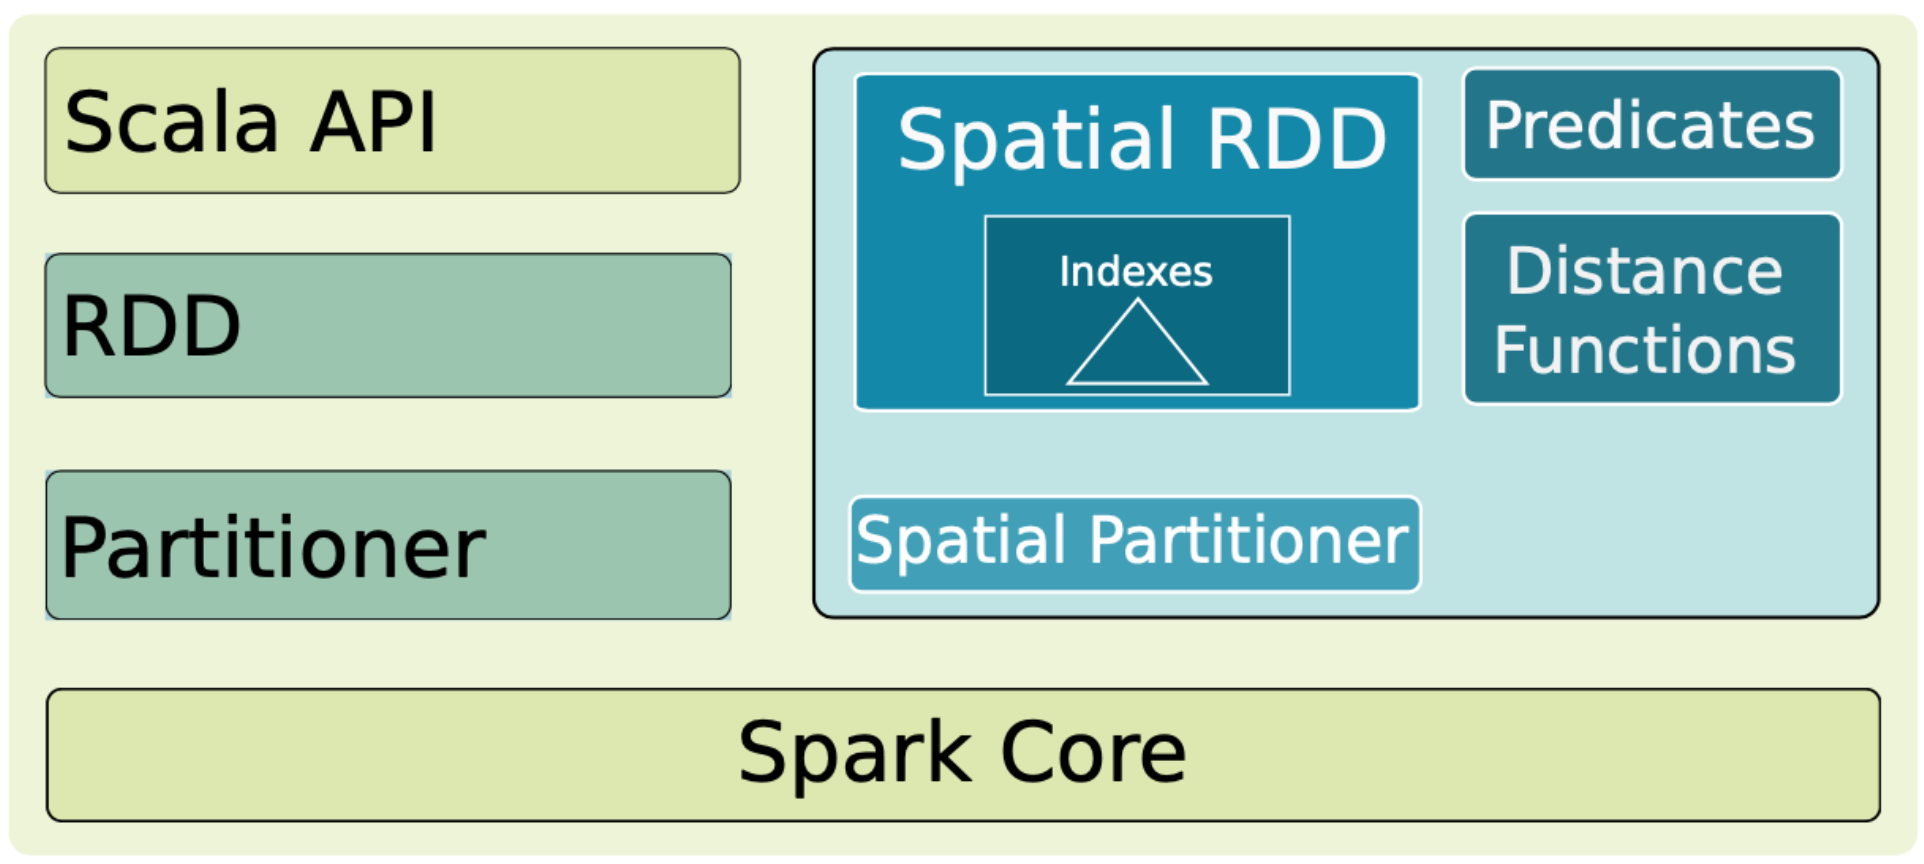
\includegraphics[width=0.8\textwidth]{images/stark_arch.png}
	\caption{Overview of STARK architecture and integration into Apache Spark \cite{article:stark}}
	\label{fig:stark_arch}
\end{figure}

To add support of spatio-temporal operators to standard RDDs and to work with spatio-temporal data, STARK implements following classes: STObject, SpatialRDD. STObject is a basic data structure in STARK. It is used to represent the spatial or spatio-temporal component of any object and has two fields: 1) $geo$ to store the spatial data and 2) $time$ to store the temporal component. Also STObject class provides operations to test relations between instances: $intersect(o)$, $contains(o)$, $containedBy(o)$. A SpatialRDD is intended to store spatio-temporal vector data sets. Figure \ref{fig:stark_arch_2} shows the architecture of STARK framework with emphasizing added functionality.

\begin{figure}[!htb]
	\centering{}
	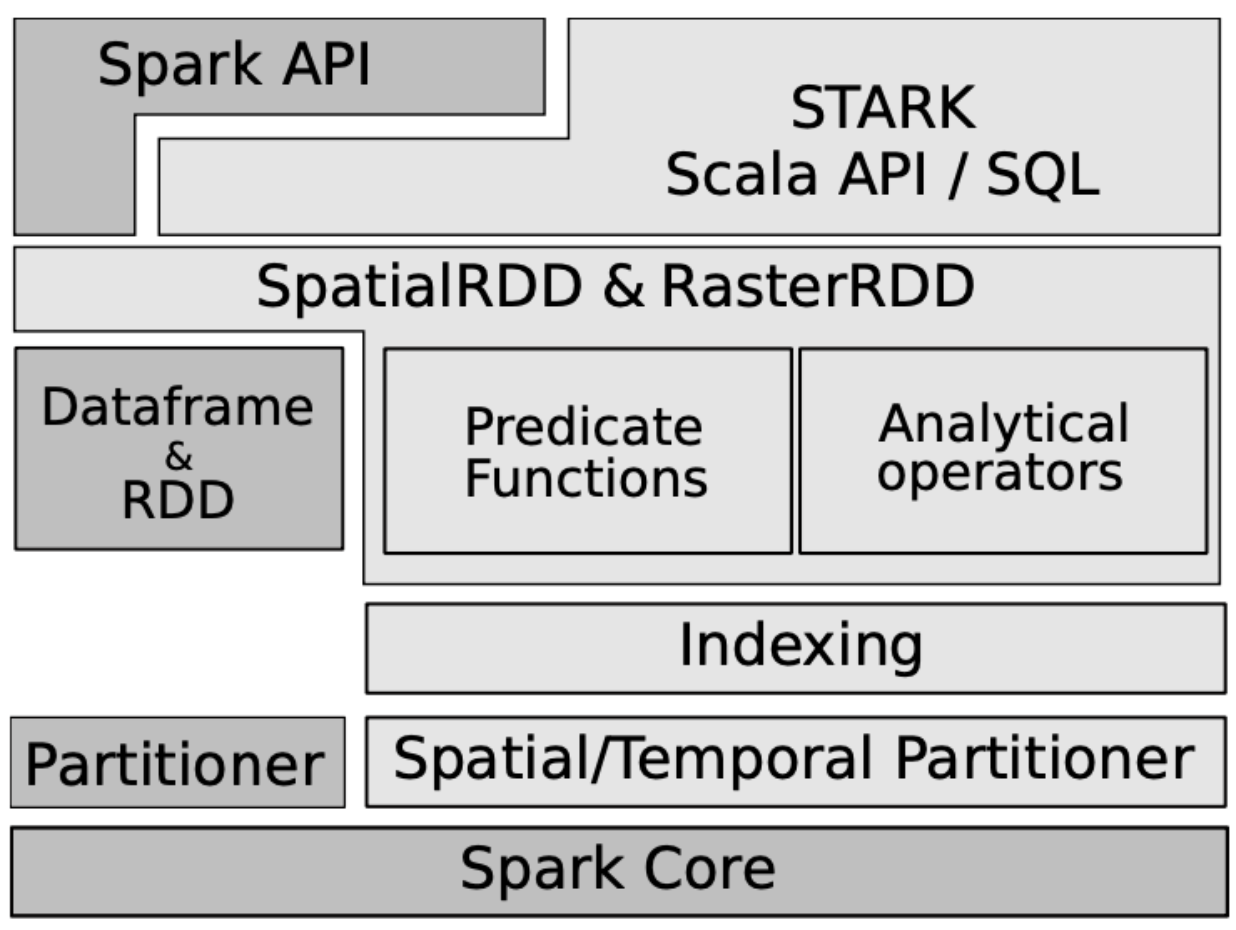
\includegraphics[width=0.8\textwidth]{images/stark_arch_2.png}
	\caption{Detailed STARK architecture \cite{article:stark_raster}}
	\label{fig:stark_arch_2}
\end{figure}


\subsection{Summary}

According to the aforegoing description, it was decided to use following technologies for implementation part of the thesis work:
\begin{itemize}
	\item Apache Spark is chosen as a base platform for implementation, since it offers higher performance in comparison with Apache Hadoop and has powerful extensions.
	\item  STARK framework is chosen to perform operations on spatio-temporal trajectory data, since Apache Spark natively lacks support for spatio-temporal data processing.
\end{itemize}


